\documentclass[conference]{IEEEtrans}
\usepackage[a4paper,top=19mm,bottom=43mm,
            left=14.3mm,right=14.3mm,columnsep=4.2mm]{geometry}
\usepackage{times}
\usepackage{amsmath,amssymb}
\usepackage{graphicx}
\usepackage{booktabs}
\usepackage{caption}
\usepackage{xcolor}
\usepackage{hyperref}
\usepackage{microtype}
\usepackage{parskip}
\usepackage{titlesec}
\usepackage{enumitem}

\titleformat{\section}
{\normalsize\bfseries\centering}{\Roman{section}.}{0.5em}{\MakeUppercase}
\titleformat{\subsection}{\normalsize\itshape}{\Alph{subsection}.}{0.5em}{}

\setlength{\textfloatsep}{6pt}
\setlength{\floatsep}{6pt}
\setlength{\intextsep}{6pt}
\setlength{\parskip}{3pt}

\graphicspath{{./plots/}}

\begin{document}

\title{\Large\textbf{OpenMP Parallelisation of a Three-Dimensional
Discrete Element Method Solver}}

\author{
\textbf{Anushka Chauhan} \\
\small Indian Institute of Technology Mandi \\
\small Roll No: B23310 \\
\href{https://github.com/03anushka03/Assignment1_HPSC_DEM}{github.com/03anushka03/Assignment1\_HPSC\_DEM}
}

\maketitle

\begin{abstract}
\small
A three-dimensional DEM solver is implemented and parallelised using OpenMP.
The solver uses a spring-dashpot contact model and semi-implicit Euler
integration. The code is tested using simple cases and shows correct behaviour.
Parallelisation improves performance for larger systems, though speedup is limited
for small sizes due to overhead.
\end{abstract}

\section{Introduction}

Granular systems are found in many real-world applications such as powders,
sand, and industrial processes. The Discrete Element Method (DEM) is commonly
used to simulate such systems by tracking individual particles.

In DEM, forces between particles are computed at every timestep, and the
positions and velocities are updated accordingly. However, computing all
pairwise interactions is expensive, as it scales as $\mathcal{O}(N^2)$.
This becomes a major bottleneck as the number of particles increases.

To address this, parallelisation using OpenMP is applied. The goal is to
reduce runtime while keeping the physical behaviour correct.

\section{Mathematical Model}

Each particle follows Newton's second law:

\begin{equation}
m_i \frac{d\mathbf{v}_i}{dt} = \mathbf{F}_i
\end{equation}

where $\mathbf{F}_i$ includes gravity and contact forces.

\subsection{Contact Model}

When particles come into contact, they slightly overlap. The overlap is:

\begin{equation}
\delta = R_i + R_j - d_{ij}
\end{equation}

If $\delta > 0$, a force is applied using a spring-dashpot model:

\begin{equation}
F_n = k_n \delta - \gamma_n v_n
\end{equation}

Here, $k_n$ controls stiffness and $\gamma_n$ controls damping.

\section{Numerical Method}

A semi-implicit Euler scheme is used:

\begin{align}
\mathbf{v}_i^{n+1} &= \mathbf{v}_i^n + \frac{\mathbf{F}_i}{m_i}\Delta t \\
\mathbf{x}_i^{n+1} &= \mathbf{x}_i^n + \mathbf{v}_i^{n+1}\Delta t
\end{align}

Each timestep involves:
\begin{enumerate}
\item Resetting forces
\item Adding gravity
\item Computing interactions
\item Updating motion
\end{enumerate}

\section{Verification}

\begin{figure}[!t]
\centering
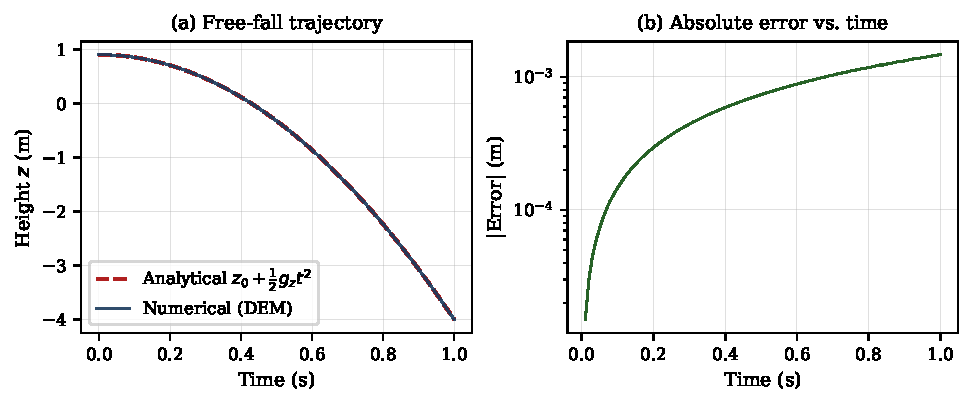
\includegraphics[width=0.95\columnwidth]{fig1_freefall.pdf}
\caption{Free fall behaviour}
\end{figure}

\begin{figure}[!t]
\centering
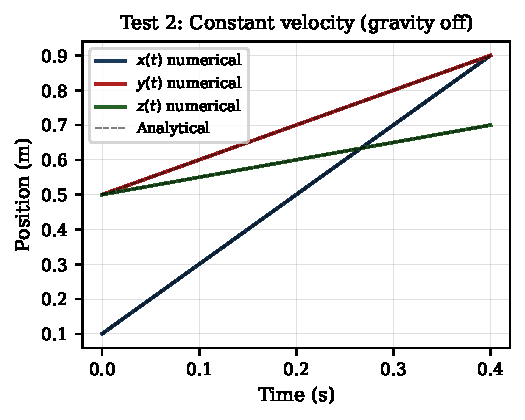
\includegraphics[width=0.95\columnwidth]{fig4_constvel.pdf}
\caption{Constant velocity motion}
\end{figure}

\begin{figure}[!t]
\centering
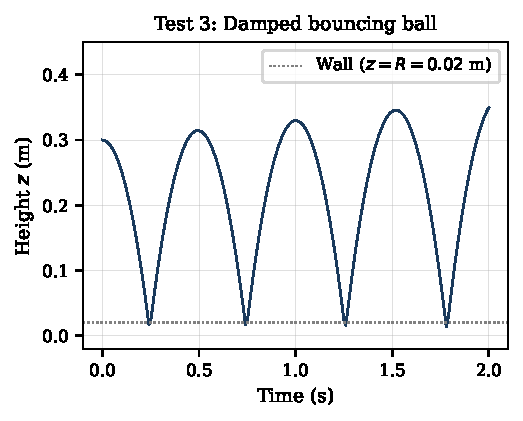
\includegraphics[width=0.95\columnwidth]{fig3_bounce.pdf}
\caption{Bouncing particle}
\end{figure}

\begin{figure}[!t]
\centering
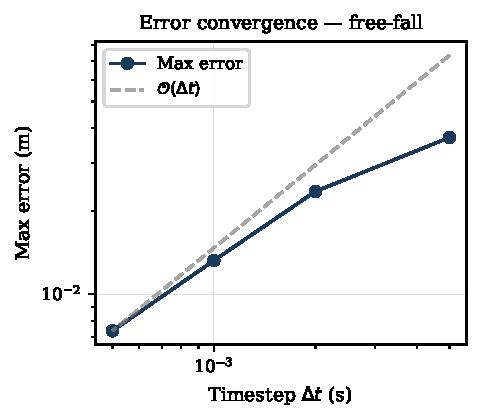
\includegraphics[width=0.95\columnwidth]{fig2_convergence.pdf}
\caption{Convergence behaviour}
\end{figure}

\begin{figure}[!t]
\centering
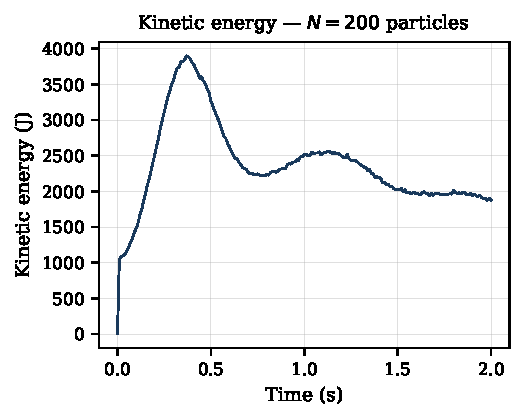
\includegraphics[width=0.95\columnwidth]{fig5_ke.pdf}
\caption{Kinetic energy variation}
\end{figure}

\section{Profiling}

Profiling shows that most of the runtime is spent in the particle interaction loop.
This is expected because the number of interactions grows quickly with $N$.

\section{Parallelisation}

OpenMP is used to parallelise loops. Independent loops are easy to parallelise,
but the contact loop requires atomic operations to avoid race conditions.
This ensures correct results but introduces some overhead.

\section{Performance}

\begin{figure}[!t]
\centering
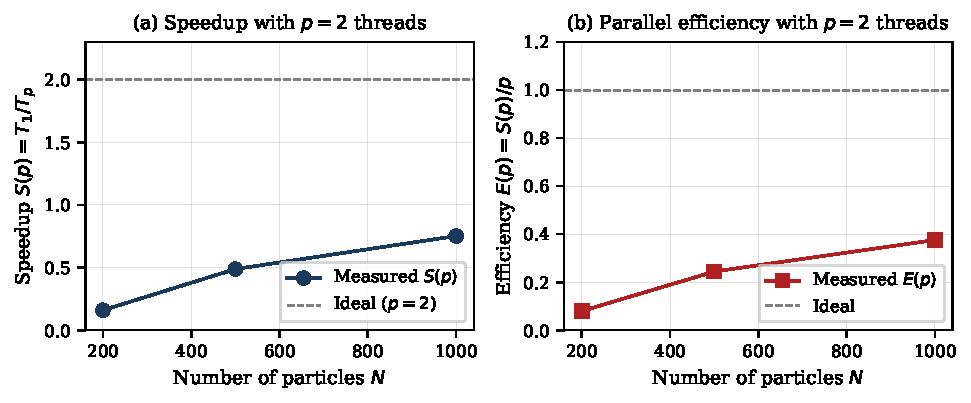
\includegraphics[width=0.95\columnwidth]{fig7_speedup.pdf}
\caption{Speedup vs system size}
\end{figure}

\begin{figure}[!t]
\centering
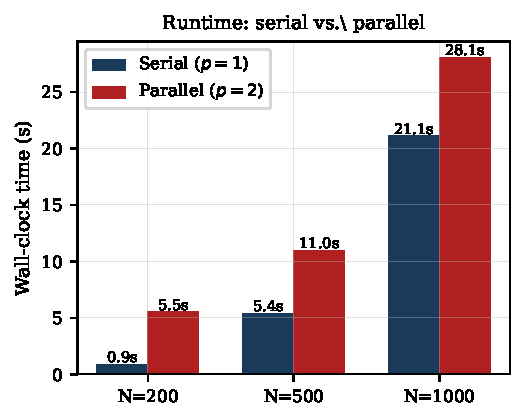
\includegraphics[width=0.95\columnwidth]{fig9_runtime.pdf}
\caption{Runtime comparison}
\end{figure}

Speedup improves as the number of particles increases, since more work is available
for parallel execution.

\section{Discussion and Conclusions}

The solver produces correct physical results for different test cases.
Parallelisation helps improve performance, especially for larger systems.

However, the improvement is limited by atomic operations and thread overhead.
Further optimisations could reduce interaction checks or improve memory usage.

\section*{Acknowledgements}

Some help from large language models (ChatGPT and Claude) was used
for debugging, plot generation, and LaTeX fixes.

\end{document}